\documentclass{BachelorBUI}
\usepackage[utf8]{inputenc}
\RequirePackage[babel,english=american]{csquotes} %% context sensitive quotations
\raggedbottom
\lstset{
 language={Matlab},
}
\sisetup{output-decimal-marker = {,},
range-phrase = --,
group-separator = {~},
per-mode = symbol,
list-final-separator={ and }}

%----------------------------------------------------------------------------------------
% Packages
%----------------------------------------------------------------------------------------
\usepackage{tikz}
\usepackage{color}
\usetikzlibrary{positioning, shapes.multipart}

%----------------------------------------------------------------------------------------
% Graphics
%----------------------------------------------------------------------------------------
\graphicspath{{images/}}

%----------------------------------------------------------------------------------------
% New commands and other new definitions (e.g. colors)
%----------------------------------------------------------------------------------------
\newcommand{\eg}{\mbox{e.\,g.}\xspace}
\newcommand{\Name}[1]{\textsc{#1}}
\newcommand{\abs}[1]{\left|#1\right|}
\colorlet{light_grey}{gray!25}
\colorlet{dark_grey}{light_grey!50!black}
\colorlet{light_red}{red!25}
\colorlet{dark_red}{light_red!50!black}
\colorlet{light_blue}{blue!25}
\colorlet{dark_blue}{light_blue!50!black}
\colorlet{light_green}{green!25}
\colorlet{dark_green}{light_green!50!black}

%----------------------------------------------------------------------------------------
% Acronyms
%----------------------------------------------------------------------------------------
\usepackage{acro}
\acsetup{list/display=used}
\input{acronyms}

%----------------------------------------------------------------------------------------
% Settings of document structure depth
%----------------------------------------------------------------------------------------
\setcounter{secnumdepth}{3}
\setcounter{tocdepth}{3} 

%----------------------------------------------------------------------------------------
% Bibliography
%----------------------------------------------------------------------------------------
\usepackage[style=authoryear,backend=biber,maxcitenames=2]{biblatex}
\ExecuteBibliographyOptions{%
 giveninits=true, maxbibnames=99}%
\DefineBibliographyStrings{english}{%
andothers={et\;al\adddot},
urlseen = {Accessed on}
}
\addbibresource{references.bib}
\setcounter{biburllcpenalty}{9000}% Lowercase
\setcounter{biburlucpenalty}{9000}% Uppercase

%----------------------------------------------------------------------------------------
% Title and author information
%----------------------------------------------------------------------------------------
\title{Plant Disease Classification:\\[0.5em]\LARGE An Approach using Convolutional Neural Networks}
\authorname{Jakub Dunaj} 
\email{e12121285@student.tuwien.ac.at} 
\MatrNr{12121285} 
\thesislanguage{en-US} 
\keywords{bachelor's thesis\sep plant disease classification\sep convolutional neural networks\sep CNNs\sep}

%----------------------------------------------------------------------------------------
% Begin of the document
%----------------------------------------------------------------------------------------
\begin{document}
\selectlanguage{english}
\begin{filecontents}[overwrite]{\jobname.xmpdata}
\makeatletter
\Title{\@title}
\Author{\@authorname}
\Language{\@thesislanguage}
\Keywords{\@keywords}
\Publisher{TU Wien}
\makeatother
\end{filecontents}

%----------------------------------------------------------------------------------------
% Title
%----------------------------------------------------------------------------------------
\maketitle

%----------------------------------------------------------------------------------------
% Abstract
%----------------------------------------------------------------------------------------
\begin{abstract}
\end{abstract}

%----------------------------------------------------------------------------------------
% Table of contents
%----------------------------------------------------------------------------------------
\clearpage
\tableofcontents

%----------------------------------------------------------------------------------------
% Bachelor's thesis
%----------------------------------------------------------------------------------------
\clearpage
\section{Introduction}

\section{Thesis Focus and Related Work}

    \subsection{Machine Learning: An Introduction}
    \label{sec:machine-learning-overveiw}

        I want the reader of my thesis to think about a random sequence of characters 'd' and 'f'. The reader can try to write down a random sequence of maybe 10 to 20 of these two characters. How random does the reader think the sequence is? Are there any patterns present in the sequence? In fact, this is hard to tell only from one short sequence. What about thousand sequences or one very long sequence? Does the reader think that those would be random and unique even if she or he tried very hard? I would advise the reader to have a look at the following website \url{https://people.ischool.berkeley.edu/~nick/aaronson-oracle/index.html} and try the website out. The algorithm on the website attempts to predict whether the next typed character will be 'd' or 'f'. The algorithm predicts the next typed character based on the sequence of 'd's and 'f's the user has typed so far. In \autoref{fig:website-predicting-typed-characters}, the algorithm could predict my next typed character with a probability of 67\%. 

        \begin{figure}[h]
            \centering
            \includegraphics[width=0.8\textwidth]{website_predicting_typed_characters.png}
            \caption{Website predicting whether the user will type 'd' or 'f' next (\cite{website_predicting_typed_characters:2024})}
            \label{fig:website-predicting-typed-characters}
        \end{figure}

        The website is based on the book "Quantum Computing since Democritus" by Scott Aaronson. \textcite{Aaronson:2013} wrote a simple program predicting whether the next typed character would be 'd' or 'f'. The author found that the algorithm was successful 70\% of the time. To answer the rhetorical questions asked at the beginning of this sections, humans can't generate truly random sequences of 'd's and 'f's. There is something fundamental in our sequences making the next character predictable. That is true for all human-generated data. In fact, we leave patterns in all our data. This is tightly coupled with human behavior and the complexity of our everyday tasks. Humans don't behave randomly. We exercise different behavioral patters instead. We can observe this phenomenon all around us. For example, fashion trends differ between generations or age groups. Young people wear different styles of clothes than elderly people. People with higher income spend their money differently than people with lower income. Sporty people are maybe more health conscious and tend to buy healthier groceries than general population. 
        
        We can think, for example, of a large fashion retailer offering thousands of articles in thousands of physical stores and through a website. This retailer wants to know which products or styles and when are popular among customer. The retailer stores different data from every transaction made online or in-store by customers enrolled in the bonus program: customer gender, customer age, articles bought, total price, store location, current weather, current clothing season, and many others. Customers don't buy their clothes randomly. They are influenced by many different factors, such as their gender or age group. From this huge amount of collected data, the retailer could infer different behavioral patterns and accordingly modify its offer to maximize profits. The retailer could ask the following question: "What products do 35-year-old customers buy in Vienna during the summer after 2PM?". Clearly, there is no standard algorithm for this complex multidimensional problem. We don't have the knowledge about the behavioral patterns of the customers. Instead, we need to create a mechanism that would infer these patterns in customers' buying habits from the transaction data. That is where the machine learning comes into play. It allows us to predict possible outputs based on a specific input of parameters. In the specified problem, the input parameters would be the customer's age, store location, clothing season and purchase time. We would expect the mechanism to predict the customers' preferences from these input parameters. The mechanism would obtain and infer the knowledge from the transaction data.

        More formally, we can define machine learning as creating and applying computational methods using data to make accurate predictions or optimize different complex tasks (\cite{Mohri:2018}). These computational methods consist of learning algorithms processing the training data and models representing the knowledge gained from the learning process (\cite{Alpaydin:2014}). A model is defined by a set of parameters influencing model's response to a given input (\cite{Alpaydin:2014}). A model can be, for example, simple linear function or a complex model such as a neural network. During the learning process, the learning algorithm optimizes model's parameters using the training data (\cite{Alpaydin:2014}). The final trained model approximates the patterns and regularities present in the data and provides useful representation of the knowledge gained during the training process (\cite{Alpaydin:2014}). We can refer to the training data as the experience the training algorithms use to train machine learning models. A trained model may not contain all information present in the training data, but it makes predictions that are accurate enough and thus useful (\cite{Alpaydin:2014}). From the computer science perspective, there are different aspects of machine learning that have to be considered (\cite{Alpaydin:2014}). The learning algorithm must efficiently solve the optimization problem of model's parameters. There must be an efficient way to store and process large amounts of training data, and the model's algorithmic representation must be efficient as well.
        
        Machine learning is a subfield of artificial intelligence. To be and behave intelligent, a machine learning model has to have the ability to learn and adapt to the changes in the training data (\cite{Alpaydin:2014}). The changes in the training data result from the changes in the experience the data describes. The model has to adapt to these changes through learning to accurately approximate the experience. Furthermore, because of the ability of the machine learning models to learn and adapt, there is no need to program the model explicitly (\cite{Alpaydin:2014}). The trained model may be predictive, descriptive, or have both of the features at the same time (\cite{Alpaydin:2014}). This means that the model can make predictions about the future or describe the knowledge from the data, or even do both. All the model's knowledge is inferred from the training data.

        The prediction accuracy of a model depends on the size of training data and the model complexity (\cite{Murphy:2022}). A model is accurate when it can generalize well (\cite{Mohri:2018}). Generalization means that the model makes accurate predictions not only about the training data but also about unseen data (\cite{Bishop:2006}). To achieve good model generalization, a trade-off between the size of the training data and the model complexity must be done (\cite{Bishop:2006,Mohri:2018}). The model complexity can be defined as the number of parameters of the model (\cite{Bishop:2006}). When the training data is small and the model is too complex, it may generalize poorly to unseen data (\cite{Mohri:2018}). This is known as overfitting of the trained model (\cite{Mohri:2018}). On the other hand, a model that is too simple may not be able to achieve sufficient accuracy on the training data. This is known as underfitting (\cite{Mohri:2018}). 

        What kind of problems can be solved using machine learning? When do we use machine learning instead of explicitly programming a computer program? There are two aspects of the problems we have to consider. These are the complexity of the problem and the need for adaptivity of the computer program (\cite{Shalev-Shwart:2014}). Complex problems may require mimicking animal or human intelligence or even go beyond human capabilities (\cite{Shalev-Shwart:2014}). The adaptivity of the computer program is its ability to learn from a changing experience without explicit programming (\cite{Shalev-Shwart:2014}). Machine learning is used in a variety of problem settings that involve: natural language processing, speech processing, computer vision, computational biology, and many others (\cite{Mohri:2018}).

        % needs to be rewritten
        Furthermore, I want to discuss machine learning approaches and neural networks as a machine learning model. I want to give an overview of neural networks because they play a central role in this thesis. The knowledge about neural networks is very important because I want to build on this knowledge in the later parts of this thesis. % maybe adding here some other machine learning models -> Support Vector Machines (SVM), K-nearest Neighbors (KNN), Decision Trees, Random Forest, K-means Clustering

        \subsubsection{Machine Learning Approaches}
        % add mathematical representation of vectors to the text and also the model can be represented as a function so add it

            Machine learning approaches can be divided into different categories based on the type of experience machine learning algorithms use to train machine learning models (\cite{Goodfellow:2016}). The different categories of machine learning approaches are: supervised, unsupervised and reinforcement learning. These categories are groups of machine learning algorithm that use the same type of experience for the training of models. As mentioned in the previous sections, the experience is the training data used by a machine learning algorithm. Each of these categories of machine learning algorithms can be applied to different groups of learning problems. Next, I want to discuss the different categories of machine learning algorithms and also the groups of learning problems the categories of algorithms are used for.
    
            \paragraph{Supervised Learning}
                
                In supervised learning, the objective is to train a machine learning model using labeled training data to map an input to a correct output (\cite{Alpaydin:2014}). This learning approach is called supervised because the training data consists of input--output pairs (\cite{Murphy:2022}). This means that the output is known for every input. The input of a machine learning algorithm is called a feature, which is typically a fixed-dimensional vector of numbers (\cite{Murphy:2022}). The output of a trained model is typically also a fixed-dimensional vector (\cite{Bishop:2006}). A machine learning algorithm uses the input vector from the problem instance to train a model that maps this input to an output vector (\cite{Bishop:2006}). An output that is associated with an input is also known as a label (\cite{Murphy:2022}). During a supervised learning process of a machine learning model, a machine learning algorithm tries to minimize the approximation error between the true label and the label predicted by the trained model (\cite{Alpaydin:2014}). A machine learning algorithm does this by adjusting the parameters of the trained model (\cite{Alpaydin:2014}). A feature used by a machine learning algorithm could be a vector of values representing pixels of an image (\cite{Murphy:2022}). The label of such an input vector could be the name of an object that is represented in the image. 

                There are two different groups of machine learning problems that can be solved using a supervised learning approach: classification and regression problems. In classification problems, every problem instance belongs to a class. The task in classification problems is the prediction of the class of a problem instance (\cite{Goodfellow:2016}). In supervised learning, the problem instance and its associated class build the input--output pair. The output of a machine learning model trained to solve a classification problem is typically a probability distribution over all classes occurring in the problem setting (\cite{Goodfellow:2016}). Classification problems could be simple binary classification problems or problems involving many different discrete classes. There are different examples of classification problems: pattern recognition, face recognition, medical diagnosis, speech recognition, natural language processing, biometrics, knowledge extraction, outlier detection, or for example novelty extraction (\cite{Alpaydin:2014}). For example, a medical diagnosis problem would be predicting a disease based on a patient's medical status. The input vector could contain the patient's age, gender, current health issues, or past medical history. The machine learning model would then predict the disease based on this information.

                Regression problems are problems of predicting one or more continuous variables for a problem instance (\cite{Bishop:2006}). An example of a regression problem would be the price prediction for a used car (\cite{Alpaydin:2014}). The input vector could contain the car's brand, year, mileage, fuel consumption, or color. The label of this input would then be the price for the specific car. The input--output pairs in training data would consist of car features and prices. Another regression problem would be the prediction of company stock prices based on different markers describing the company's performance (\cite{Mohri:2018}).

            \paragraph{Unsupervised Learning}

                Supervised machine learning algorithms use labeled training data to create a machine learning models that map the inputs  to learned outputs. In unsupervised learning, the training data consists only of fixed-dimensional input vectors without any labels (\cite{Bishop:2006}). The objective of unsupervised learning is to find regularities in the training data (\cite{Alpaydin:2014}). In unsupervised learning, learning algorithms use only the input vectors from the unlabeled training data to train model that are able to find regularities or structures in the input space (\cite{Alpaydin:2014}). There are various groups of machine learning problems that can be solved using an unsupervised machine learning approach. The partitioning of problem instances into homogeneous subsets is called clustering (\cite{Mohri:2018}). An example of a clustering problem is image compression (\cite{Alpaydin:2014}). A machine learning algorithm would search for clusters of pixels with similar colors. The average pixel color for the pixel regions is then computed. Saving information only about the location of the pixel regions and about the average color of the regions compresses the size of an image. Another group of problems is the dimensionality reduction problems (\cite{Mohri:2018}). If the problem instances have a large number of parameters, so that the input vectors are of high dimension, there is often a need to search for lower-dimensional representation of problem instances (\cite{Mohri:2018}). The high dimensionality of input vectors is reduced to speed up computations done on the data or to extract only parameters of problem instances that are useful and significant (\cite{Mohri:2018}). 

            \paragraph{Reinforcement Learning}

                In reinforcement learning, a learning algorithm tries to find a solution, sequence of actions, to a problem by interacting with the environment (\cite{Alpaydin:2014}). In contrast to supervised or unsupervised learning algorithms, a reinforcement learning algorithm does not have any prepared training data to use to find the best sequence of actions (\cite{Mohri:2018}). Instead, the learning algorithm, also called learner or agent, collects the data by exploring an environment using the trial and error process (\cite{Bishop:2006}). When interacting with the environment, the agent receives rewards or penalties for its actions (\cite{Alpaydin:2014}). Based on the rewards or penalties, the learner tries to modify its future actions to maximize the reward (\cite{Mohri:2018}). By maximizing the reward, the learner searches for the optimal solution to a given problem (\cite{Bishop:2006}). The resulting sequence of actions leading to the optimal solution is also called a policy. The reward or penalty that the learner receives is only for its immediate action (\cite{Mohri:2018}). That is why the learner has to learn from its past actions to assess and predict how its future action may influence the goodness of the current policy (\cite{Alpaydin:2014}). This is also called the exploration versus exploitation dilemma (\cite{Alpaydin:2014}). The learner has to decide between exploring the environment to gain more information and exploiting the information it has already collected (\cite{Alpaydin:2014}). An example of a problem that can be solved by a reinforcement learning algorithm is teaching a learner to play chess (\cite{Alpaydin:2014}). There are about $10^{120}$ different possible chess games (\cite{Shannon:1988}). It is computationally infeasible to use supervised or unsupervised learning approach and list all of the possible piece positions or games. In reinforcement learning setting, one move done by the learner leaning to play chess in insignificant on itself. The learner receives the feedback after completing the whole game. Receiving reward or penalty depends on winning or losing a game. This means that the learner learns the goodness of the complete sequence of moves.

        \subsubsection{Neural Networks: An Introduction}

            Neural networks are machine learning models that are inspired by the biological nervous systems, in particular the central nervous system of humans (\cite{Aggarwal:2018}). The building unit of the human central nervous system is a cell called neuron. \autoref{fig:anatomy-of-neuron} shows the anatomy of a neuron. Two different types of wire-like connections to other neurons originate at the soma of a neuron (\cite{Gerstner:2014}). The soma contains the neuron's nucleus. The dendrites are one of these two types. Dendrites form a branched structure from the surface of neuron's soma. Through contact points on the dendrites, referred to as synapses, a neuron receives signals from other neurons (\cite{Gerstner:2014}). The strength of the synaptic connections modifies the response of the neuron to external stimuli (\cite{Aggarwal:2018}). The other type of these connections is the axon. An axon also forms a branched structure at its end. A neuron uses the axon to send signals to other neurons (\cite{Gerstner:2014}). The soma and the initial segment of an axon can stimulate or prohibit the signal transmission to other connected neurons (\cite{Gerstner:2014}). 
            
            As response to stimuli from sending neurons, the strength of the synaptic connections of the receiving neurons changes (\cite{Aggarwal:2018}). The sending neuron is also referred to as presynaptic neuron and the receiving neuron is referred to as postsynaptic (\cite{Gerstner:2014}). If a presynaptic neuron fires frequently, the synaptic connections of the postsynaptic neuron strengthen (\cite{Aggarwal:2018}). If a presynaptic neuron is excited sparsely, the synaptic connections of the postsynaptic neuron weaken (\cite{Aggarwal:2018}). This is the core process how learning takes place in biological nervous systems (\cite{Aggarwal:2018}). 

            \autoref{fig:schematic-anatomy-of-neuron} shows a schematic anatomy of a neuron. We can analyze the neuron's structure from a computer science perspective. The dendrites play a role of an input device that leads the signal from presynaptic neurons to the soma of a postsynaptic neuron (\cite{Gerstner:2014}). In \autoref{fig:schematic-anatomy-of-neuron}, these input devices are modeled as $x_1, x_2, x_3, \dots, x_n$. The importance of a signal is determined by the strength of the synaptic connections in postsynaptic neurons. The strength of a synaptic connection can be modeled as its weight to the whole neuron's input (\cite{Gerstner:2014}). In \autoref{fig:schematic-anatomy-of-neuron}, every input device $x_i$ has an assigned weight $w_i$ that scales the input signal. The soma plays a role of a central computing unit of a neuron (\cite{Gerstner:2014}). It executes a nonlinear computing step (\cite{Gerstner:2014}). It generates and passes a signal through the neuron's axon when a certain strength threshold of incoming signals is exceeded (\cite{Gerstner:2014}). The axon can be described as an output device of the neuron sending signals to other neurons (\cite{Gerstner:2014}). We can consider the biological neuron as a computing device that receives incoming signals, considers the incoming signals together with their wights and applies some activation function. This activation function considers the combined strength of all weighted incoming signals. Is a certain threshold value achieved, the neuron as a computing device forwards the signal to all connected neurons. This analogy of biological neurons in computer science laid the fundamental ground for the development of artificial neurons and artificial neural networks. An artificial neuron scales the incoming inputs using a weight and then applies an activation function to the combined input (\cite{Aggarwal:2018}). An artificial neural network propagates the input values through its layers (\cite{Aggarwal:2018}). By propagating the input values through the network and by using the weights as intermediate parameters, the artificial neural network computes a function of the input values (\cite{Aggarwal:2018}). The learning takes place by changing the weights of incoming inputs (\cite{Aggarwal:2018}). The weights of the incoming inputs are adjustable parameters of the neural network (\cite{LeCun:2015}). The learning process of neural networks may be supervised or unsupervised (\cite{Aggarwal:2018,LeCun:2015}). The prevalent learning approach is supervised (\cite{LeCun:2015}).

            \begin{figure}[h]
                \begin{subfigure}[b]{0.49\textwidth}
                    \centering
                    \includegraphics[width=\textwidth]{anatomy_of_neuron.png}
                    \caption{Anatomy of a neuron (Source: \cite{anatomy_of_neuron:2022})}
                    \label{fig:anatomy-of-neuron}
                \end{subfigure}
                \hfill
                \begin{subfigure}[b]{0.49\textwidth}
                    \centering
                    \resizebox{\textwidth}{!}{
                        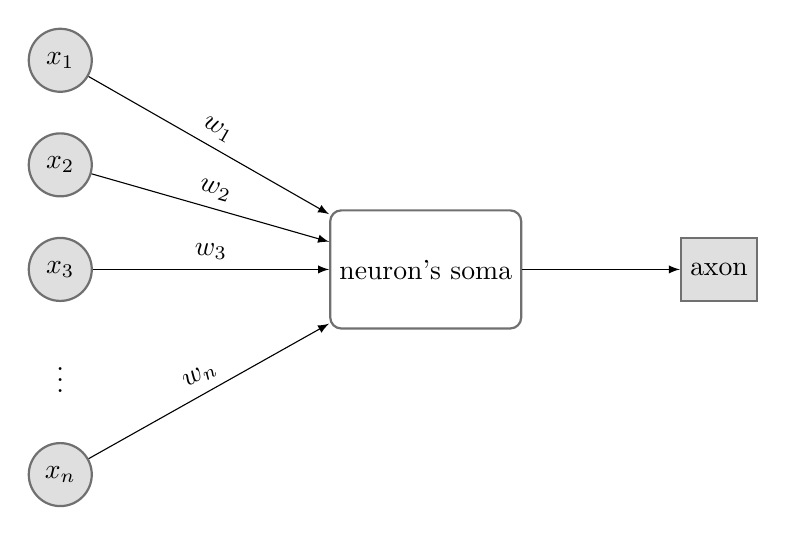
\begin{tikzpicture}[
                            neuron/.style={rectangle, draw=dark_grey, rounded corners, minimum width=2cm, minimum height=1.5cm, thick},
                            input/.style={circle, draw=dark_grey, fill=light_grey, minimum size=0.8cm, thick},
                            output/.style={rectangle, draw=dark_grey, fill=light_grey, minimum size=0.8cm, thick},
                            node distance=0.5cm and 3cm,
                            >=latex,
                            transform shape
                        ]
                            % nodes
                            \node[input] (x1) at (0,0){$x_1$};
                            \node[input] (x2) [below=of x1]{$x_2$};
                            \node[input] (x3) [below=of x2]{$x_3$};
                            \node (dots) [below=0.5cm of x3] {$\vdots$};
                            \node[input] (xn) [below=of dots]{$x_n$};
                            \node[neuron] (neuron) [right=of x3] {neuron's soma};
                            \node[output] (output) [right=2cm of neuron] {axon};

                            % connections
                            \draw[->] (neuron) -- (output);
                            \foreach \i in {1,2,3,n} {
                                \draw[->] (x\i) -- (neuron)
                                    node[pos=0.5, sloped, above]{$w_\i$};
                            }
                        \end{tikzpicture}
                    }
                    \caption{Schematic anatomy of a neuron (Adapted from: \cite{Aggarwal:2018})}
                    \label{fig:schematic-anatomy-of-neuron}
                \end{subfigure}
                \caption{Detailed and schematic anatomy of a neuron}
            \end{figure}

            The artificial neuron is a basic processing unit and a building block of artificial neural networks (\cite{Alpaydin:2014}). At the same time, single artificial neuron builds a single-layer neural network. Single-layer networks may also include several artificial neurons in parallel. Layers of artificial neurons build complex neural networks that are also referred to as multilayer neural networks. Neural networks use representation learning (\cite{LeCun:2015}). This means that the artificial neural network discover the patterns in the data automatically without preprocessing the raw data (\cite{LeCun:2015}). The neural networks learn different representations of the input data at each of the layers (\cite{LeCun:2015}). The preprocessing of the raw data to extract important features has to be done in some conventional machine-learning approaches such as K-Nearest Neighbors technique.
            
            In the following paragraphs, I want to describe and provide insights into the single-layer and multilayer neural networks. 
            
            \paragraph{Single-layer Neural Networks}
            \label{par:single-layer-neural-networks}
                \autoref{fig:artificial-neuron} describes the structure of an artificial neuron. The input values of an artificial neuron define a vector $\mathbf{x} = [x_1 \cdots x_N]^T$, where $x_j \in \mathbb{R}$ and $j \in \{1, \cdots, N\}$ (\cite{Alpaydin:2014}). The $N$ describes the total number of input values of an artificial neuron. The associated weights for each of the input values also define a vector $\mathbf{w_i}^T = [w_{i,1} \cdots w_{i,N}]^T$, where $w_{i,k} \in \mathbb{R}$, $k \in \{1, \cdots, N\}$ (\cite{Alpaydin:2014}). The $i$ denotes the index of an artificial neuron within the single-layer neural network. The bias $b_i$ is used to make the computation of an artificial neuron more general (\cite{Alpaydin:2014}). It adds fixed offset to the input of the artificial neuron (\cite{Bishop:2024}). We can add the bias to the $\mathbf{x}$ and $\mathbf{w_i}$ vectors. We obtain the extended vectors $\mathbf{x} = [1, x_1 \cdots x_N]^T$ and $\mathbf{w_i}^T = [b_i, w_{i,1} \cdots w_{i,N}]^T$. The artificial neuron performs the dot product of the vectors $\mathbf{w_i}^T$ and $\mathbf{x}$ (\cite{Alpaydin:2014}). The dot product of the vectors as matrix multiplication is defined as:
                \begin{equation}
                    \mathbf{w_i}^T\mathbf{x} = \sum_{n=1}^{N+1} w_{i,n} x_n = w_{i,1} + w_{i,2}x_2 + w_{i,3}x_3 + \cdots + w_{i,N+1} x_{N+1}.
                    \label{eq:dot-product-complex}
                \end{equation} 
                In \autoref{eq:dot-product-complex}, the summand $w_{i,1}$ equals to $b_i$. We can reflect this and modify the \autoref{eq:dot-product-complex}. We get the following modified equation:
                \begin{equation}
                    \mathbf{w_i}^T\mathbf{x} = \sum_{n=2}^{N+1} w_{i,n} x_n + b_i.
                    \label{eq:dot-product-complex-modified}
                \end{equation} 
                In \autoref{fig:artificial-neuron}, the symbol $\sum$ represents the summation operation that computes the dot product of the input vector and its associated weight vector as matrix multiplication. Further, the artificial neuron applies an activation function to the result of the dot product. This operation is defined as:
                \begin{equation} 
                    y_{a_{i}} = f(\mathbf{w_i}^T\mathbf{x}).
                    \label{eq:activation-function-complex}
                \end{equation}
                The result of \autoref{eq:activation-function-complex} denoted as $y_{a_{i}}$ represents the output value of the artificial neuron with the index $i$ within the layer $l$.The activation function is denoted as $f$ in \autoref{fig:artificial-neuron}.

                \begin{figure}[h]
                    \centering
                    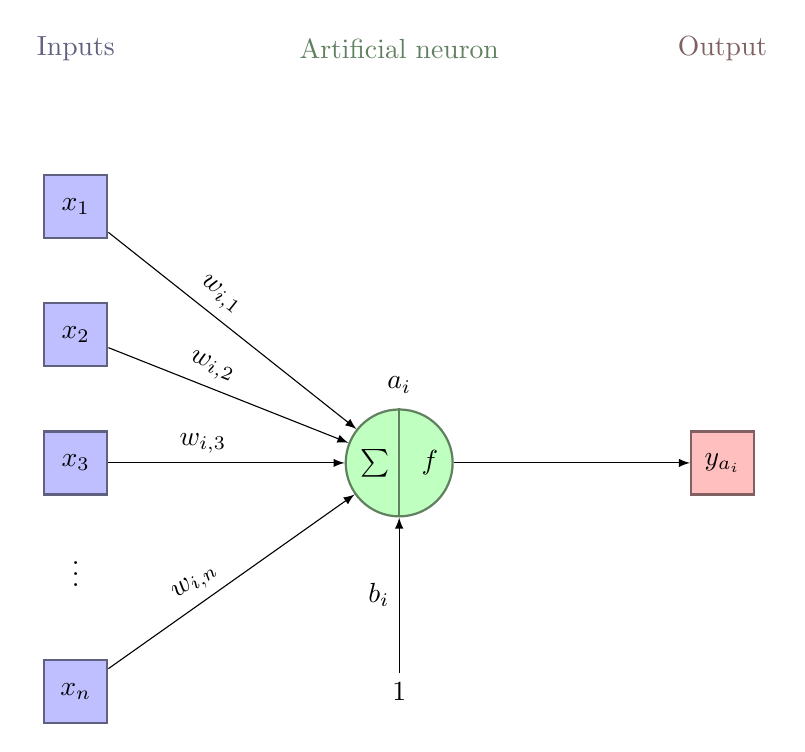
\begin{tikzpicture}[
                        input/.style={draw=dark_blue, fill=light_blue, thick, minimum size=0.8cm},
                        neuron/.style={circle, draw=dark_green, fill=light_green, minimum size=1cm, thick},
                        output/.style={draw=dark_red, fill=light_red, thick, minimum size=0.8cm},
                        node distance=0.8cm and 3cm,
                        >=latex,
                    ]
                        \coordinate (top) at (0,2);

                        %nodes
                        \node[input] (x1) at (0,0){$x_1$};
                        \node[input] (x2) [below=of x1]{$x_2$};
                        \node[input] (x3) [below=of x2]{$x_3$};
                        \node (dots) [below=0.5cm of x3] {$\vdots$};
                        \node[input] (xn) [below=of dots]{$x_n$};
                        \node[neuron] (artificial_neuron) [right=of x3]{$\sum$ \hspace{0.5em} $f$};
                        \draw[thick, draw=dark_green] (artificial_neuron.north) -- (artificial_neuron.south); % artificial neuron
                        \node[above=0.2em of artificial_neuron] {$a_{i}$}; % artificial neuron
                        \node (bias) at (artificial_neuron |- xn) {$1$};
                        \node[output] (output) [right=of artificial_neuron] {$y_{a_{i}}$};

                        % labels
                        \node[dark_blue] (inputs_label) at (x1 |- top) {Inputs};
                        \node[dark_green] (artificial_neuron_label) at (artificial_neuron |- top) {Artificial neuron};
                        \node[dark_red] (output_label) at (output |- top) {Output};
                        
                        % connections
                        \foreach \m in {1,2,3,n} {
                            \draw[->] (x\m) -- (artificial_neuron)
                                node[pos=0.4, sloped, above] {$w_{i,\m}$};
                        }
                        \draw[->] (artificial_neuron) -- (output);
                        \draw[->] (bias) -- (artificial_neuron) node[midway, left] {$b_i$};
                    \end{tikzpicture}
                    \caption{Artificial neuron (Adapted from: \cite{Aggarwal:2018})}
                    \label{fig:artificial-neuron}
                \end{figure}

                % activation functions
                Artificial neurons may use different activation functions depending on the task they should accomplish (\cite{Aggarwal:2018}). In the following examples of activation functions I will denote the dot product from \autoref{eq:dot-product-complex-modified} simply as $x$. The most basic activation function is the identity function (\cite{Aggarwal:2018}):
                \begin{equation}
                    f(x)=x.
                    \label{eq:identity-function}
                \end{equation}
                Other activation functions are (\cite{Aggarwal:2018}): the sign function
                \begin{equation}
                    f(x)=\text{sign}(x),
                    \label{eq:sign-function}
                \end{equation}
                the sigmoid function
                \begin{equation}
                    f(x) = \frac{1}{1 + e^{-x}},
                    \label{eq:sigmoid-function}
                \end{equation}
                the hyperbolic tangent function (tanh)
                \begin{equation}
                     f(x) = \frac{e^{2x}-1}{e^{2x}+1},
                    \label{eq:tanh-function}
                \end{equation}
                and the rectified linear unit function (ReLU)
                \begin{equation}
                    f(x) = \max(0, x).
                    \label{eq:relu-function}
                \end{equation}
                The sign activation function divides the input space into two half-spaces where its output is either positive or negative (\cite{Alpaydin:2014}). This function outputs either $1$ or $-1$. A single artificial neuron using the sign$(x)$ activation function, also called perceptron, can be used for binary classification (\cite{Aggarwal:2018}). While a perceptron with only one input defines a line, a perceptron with two inputs defines a plane and a perceptron with more than two inputs defines a hyperplane (\cite{Alpaydin:2014}). The sigmoid activation function, whose output values are from the interval $(0,1)$, is used when the output of an artificial neuron is interpreted as a probability. The tanh activation function outputs values from the interval $[-1,1]$ and the ReLU from the interval $[0, \infty)$. The sigmoid, tanh and ReLU activation functions are particularly applied in multilayer neural networks (\cite{Alpaydin:2014}). The sigmoid and tanh activation functions are saturating functions (\cite{Murphy:2022}). This means that for large positive numbers the sigmoid activation function outputs values approaching $1$. The tanh activation function outputs $1$. For large negative numbers, the sigmoid activation function outputs values approaching $0$ and the tanh activation function outputs $-1$. 

                To build and train a single-layer neural network, we have to define not only the activation but also the loss function for the artificial neurons. In supervised learning, the loss function quantifies the difference, or loss, between the expected value and the real output of the artificial neuron (\cite{Mohri:2018}). In term of unsupervised learning, the loss function measures the difference between the predicted output and original input of the neural network (\cite{Bishop:2024}). The concept of unsupervised learning becomes significant in multilayer neural networks. The \autoref{tab:single-layer-single-neuron-models} shows examples of different single-layer neural networks consisting of single artificial neuron and the activation and loss functions used in these models. The loss function represents the loss of the neuron for the training sample with the index $t$. The $y_t$ stands for the prediction and $\hat{y}_t$ for the label of the training pair.
                \begin{table}[h] 
                    \centering
                    \begin{tabular}{|c|c|c|}
                        \hline
                        model & activation function & loss function\\
                        \hline
                        perceptron with discrete output & sign function &  $\mathcal{L}_{t}(y_i, \hat{y}_t) = (y_t - sign(\hat{y}_t))^2$ \\
                        perceptron with continuous output & identity function & $\mathcal{L}_{t}(y_t, \hat{y}_t) = \max(0, -y_t \cdot \hat{y}_t)$ \\
                        linear regression & identity function & $\mathcal{L}_{t}(y_t, \hat{y}_t) = (y_t - \hat{y}_t)^2$ \\
                        logistic regression  & sigmoid function & $\mathcal{L}_{t}(y_t, \hat{y}_t) = -\text{log}(\abs{\frac{y_t}{2} -0.5 + \hat{y}_t})$ \\
                        support vector machine (SVM)& identity function & $\mathcal{L}_{t}(y_t, \hat{y}_t) = \max(0, -y_t \cdot \hat{y}_t + 1)$  \\
                        \hline
                    \end{tabular}
                    \caption{Single-layer neural network models consisting of a single artificial neuron (Adapted from: \cite{Aggarwal:2018})}
                    \label{tab:single-layer-single-neuron-models}
                \end{table}
                Perceptron with discrete output and support vector machine models may be used for binary classification (\cite{Alpaydin:2014}). Both of the models output real values. Logistic regression model may be used for the same task by predicting the probability for a positive class (\cite{Aggarwal:2018}). Linear regression model and perceptron with continuous output may be used for predicting a real-valued label of a problem instance represented as an input vector (\cite{Bishop:2024}). 

                Increasing the number of artificial neurons in a single-layer network, we extend the capabilities of a single-layer neural network. The \autoref{tab:single-layer-multiple-neuron-models} shows examples of different single-layer neural networks consisting of more than one artificial neuron. The table also shows the activation and loss function of the artificial neurons.
                \begin{table}[h]
                    \centering
                    \begin{tabular}{|c|c|c|}
                        \hline
                        model & activation function & loss function \\
                        \hline
                        multiclass perceptron & identity function &  $\mathcal{L}_{t}(\mathbf{\hat{y}}) = \max_{i:i \neq c(t)}\max(\hat{y}_i - \hat{y}_{c(t)}, 0)$ \\
                        multiclass SVM & identity function & $\mathcal{L}_{t}(\mathbf{\hat{y}}) = \sum_{i:i \neq c(t)}\max(\hat{y}_i - \hat{y}_{c(t)} + 1, 0)$ \\
                        multinomial logistic regression & softmax function & $\mathcal{L}_{t}(\mathbf{\hat{y}}) = -log(-\hat{y}_{c(t)})$ \\
                        \hline
                    \end{tabular} 
                    \caption{Single-layer neural network models consisting of multiple artificial neurons (Adapted from: \cite{Aggarwal:2018})}
                    \label{tab:single-layer-multiple-neuron-models}
                \end{table}
                All of the three models in \autoref{tab:single-layer-multiple-neuron-models} are used for multiclass classification problems. Each artificial neuron represents single class or label from the training set. The multiclass perceptron models as well as multiclass support vector machine models return real values (\cite{Aggarwal:2018}). The multinomial logistic regression models return probabilities for each of the classes represented by the neurons in the single-layer neural network. In addition, multinomial logistic regression models use the softmax activation function:
                \begin{equation}
                    y_{a_{i}}^t = \frac{e^{\mathbf{w_i}^T\mathbf{x}^t}}{\sum_{j=1}^{n} \mathbf{w_k}^T\mathbf{x}^t}.        
                    \label{eq:softmax-function}
                \end{equation}

                In \autoref{tab:single-layer-multiple-neuron-models}, the index $c(t)$ represents the index of an artificial neuron representing the true class for the training pair with index $t$. The loss function of a multiclass single-layer neural network compares the actual output of a neuron with the output of the neuron that represents the true class. The loss function of a multiclass support vector machine computes the maximum between $\hat{y}_i - \hat{y}_{c(t)} + 1$ and $0$ for each neuron representing a class that is different from the true class. The maximum values are then summed to a single loss value.

                The general rule for updating the weights of the weight vector $\mathbf{w_i}$ of an artificial neuron $a_{i}$ within a single-layer neural network can be defined as (\cite{Aggarwal:2018}):
                \begin{equation}
                    \mathbf{w_i} = \mathbf{w_i} - \alpha \cdot \frac{\partial \mathcal{L}_t}{\partial \mathbf{w_i}}.
                    \label{eq:gradient}
                \end{equation}
                The scaling factor $\alpha$ is called the learning rate (\cite{Aggarwal:2018}). The partial difference $\frac{\partial \mathcal{L}_t}{\partial \mathbf{w_i}}$ of loss function $\mathcal{L}_t$ with respect to the weights $\mathbf{w_i}$ is also called the gradient. That is why this update technique is called gradient descent. The \autoref{eq:gradient} assumes that the loss function is differentiable (\cite{Aggarwal:2018}).

                % stochastic gradient descent as optimization
                The limitation of the single-layer neural network is that they only learn or are limited by linear boundaries of the input space regardless of the activation function (\cite{Bishop:2024}). For example, the output values in single-layer classification can classify only data that are linearly separable (\cite{Bishop:2024}). This means that the data input space must be linearly separable by lines, planes or hyperplanes, depending on its dimensionality (\cite{Bishop:2024}).

            \paragraph{Multilayer Neural Networks}

                Multilayer neural networks contain more than one computational layer of artificial neurons. Typically, multilayer neural networks have input, output and multiple hidden layers. In \autoref{par:single-layer-neural-networks}, I have briefly described the limitations of single-layer neural networks.These are not limitations for multilayer neural networks. The multilayer neural networks can learn more complex patterns in the data by transforming the input space in a way that makes the data in the input space linearly separable (\cite{LeCun:2015}). This ability of neural networks is achieved by the hidden layers. More formally, the power of multilayer neural networks to explore non-linear patterns in the data comes from the repeated composition of non-linear functions over multiple layers of the network (\cite{Aggarwal:2018}). This increases the representational power of a multilayer neural network and lowers the numbers of parameters of the network (\cite{Aggarwal:2018}). Each layer of a multilayer neural network learns different representations of the input space (\cite{LeCun:2015}). The representations are obtained by combining simple representations at lower layer into abstract representations at higher layers. Through this composition of different representations very complex functions may be learned by the neural networks (\cite{Bishop:2024}). Thus, multilayer neural network are able to explore complex patterns in high-dimensional input data (\cite{LeCun:2015}). An example would be a neural network learning to classify different objects. At lower layers, the neural network learns the presence of horizontal and vertical lines. At the higher levels these representations are combined into abstract features of the objects such as edges or textures. This enables the neural networks to learn the distinguishing features of the objects and correctly classify them.
                
                Neural networks with a few hidden layers are considered shallow. Multilayer neural networks with many hidden layers are considered deep. Deep neural networks are at the forefront of neural networks research (\cite{LeCun:2015}). Nowadays, when discussing multilayer neural networks, a deep architecture with many layers is meant usually. The subfield of machine learning that deals with deep neural networks is called deep learning. At the core of deep learning, there is the representation learning (\cite{LeCun:2015}). As stated previously, it enables the deep neural networks to learn different abstractions of the input data at each of the layers by combining simple representations to get abstract representations of the input data (\cite{LeCun:2015}). The representation learning also allows to use the unlabeled data because it forces the neural network to explore structures in the data (\cite{Bishop:2024}).

                A standard deep multilayer architecture of a neural network is a stack of many layers of artificial neurons (\cite{LeCun:2015}). The deep neural network learns a non-linear mapping from a fixed-dimensional input to a fixed-dimensional output (\cite{LeCun:2015}). The information flows in a feed-forward way from the input layer, thought the hidden layers, to the output layer. At each layer of a deep neural network, the artificial neurons compute the weighted sum of the inputs from the previous layer. Artificial neurons neurons apply then a non-linear activation function to the weighted sum and forward the result to the next layer. The most common non-linear function used in deep neural networks is the rectified linear unit (ReLU) activation function described in \autoref{par:single-layer-neural-networks}. Deep neural networks are trained using the process of backpropagation. The backpropagation algorithm adjusts the incoming weights of artificial neurons at every layer of the neural network. As I mentioned in the \autoref{par:single-layer-neural-networks}, the adjustment of weights or parameters in a single-layer neural network is relatively easy. The problem in multilayer neural network is that the loss computed using a loss function at the output layer is also affected by the parameters in the previous layers. It is not sufficient to adjust the incoming weights of artificial neurons only at the output layer. The loss has to be propagated backwards to the previous layers of the neural network. The loss function is applied to an output that is a result of a composition of functions from the previous layers (\cite{Bishop:2024}). The contribution of any parameter within the neural network is the partial derivative of the loss function with respect to the parameter (\cite{Bishop:2024}). The backpropagation algorithm has to apply the chain rule to compute this contribution (\cite{Aggarwal:2018}). The parameters within the neural network will be then adjusted by their contribution and a learning factor in the same way as those in the single-layer neural networks.
            

                % %this probably to the next paragraph about multilayer neural networks
                % When training an artificial neural network, this behavior of sigmoid and tanh functions creates the vanishing gradient problem (\cite{Murphy:2022}). In the saturated regions of the functions, the gradient of the output of the function with respect to the function's input approaches $0$. Changes in higher layers are not propagated to the lower layers when training artificial neural networks (\cite{Murphy:2022}). The ReLU activation function is not affected by the vanishing gradient problem (\cite{Murphy:2022}).

                % different types of neural networks (RNN, CNN ...)
     
    % \subsection{Deep Learning: A Subset of Machine Learning} I will mention the deep learning as a paragraph of neural networks
        % \subsubsection{Deep Neural Networks} - I will just mention the CNNs here and then work with CNNs
        \subsubsection{Convolutional Neural Networks (CNNs)} 
            % \paragraph{CNN Architecture}
            \paragraph{Convolutional Layer}
            \paragraph{Pooling Layer}
            \paragraph{Fully Connected Layer}
            % \paragraph{Different CNN Architectures}
            % \paragraph{Common CNN Architectures in Plant Disease Classification}
            %     \subparagraph{AlexNet}
            % \paragraph{Transfer Learning}
            % \paragraph{Key Technologies in CNN Development}
    \subsection{Recent Advancements in Plant Disease Classification}

\section{Design}
    \subsection{CNN Model}
        \subsubsection{Model Architecture}
        \subsubsection{Dataset}
        \subsubsection{Training and Validation}
        \subsubsection{Model Evaluation}
    \subsection{Web-based Application}
        \subsubsection{Frontend Design}
        \subsubsection{Backend Design}
        
\section{Development}
    \subsection{CNN Model Training and Validation}
    \subsection{Web-based Application Development}
        \subsubsection{Frontend Development}
        \subsubsection{Backend Development}

\section{Web-based Application Walkthrough}

\section{Discussion}

\section{Conclusion}

%----------------------------------------------------------------------------------------
% References
%----------------------------------------------------------------------------------------
\clearpage
\printbibliography

\end{document}